\documentclass[12pt]{article}
% \usepackage[spanish]{babel}
% \usepackage{lipsum}
% \usepackage{natbib}
% \usepackage{graphicx}
\usepackage{analysis_orax}
\usepackage[hidelinks]{hyperref}
%------------------Document----------------------------
\usepackage{enumerate}
\usepackage[shortlabels]{enumitem}
\usepackage{fontawesome}
\begin{document}
\author{Abhishek Ulayil}
\title{Converting past R Journal articles to HTML}
%-------------------------TitlePage------------------------
%\begin{titlepage}
%\end{titlepage}

%-------------------------Content------------------------

\section{Project Proposal}

\subsection{Converting past R Journal articles to HTML}

\subsubsection{1. Project Info}
{\large\bfseries Short Project Title(30 character's) : } {R Journal article conversion}\\
\\
{\large\bfseries Project Idea : } {Converting past R Journal articles to HTML}\\
\\
{\large\bfseries Project synopsis :} R Journal team has been developing a new website, which would act as a central repository for all articles in HTML format. Since these many of the past articles were created in PDF format, its not always the best format for digital age interactive websites. Hence the past articles need to be converted into HTML through intermediate conversions. \\
\\
{\large\bfseries URL of project idea page:} \href{https://github.com/rstats-gsoc/gsoc2022/wiki/Converting-past-R-Journal-articles-to-HTML}{\color{orange}Converting past R Journal articles to HTML}
\subsubsection{2. A little bit about me}
 {\large Greetings},\\
 \\
\hspace*{3mm}My journey with programming and software development started when I pursued Bachelors in Computer Science degree. I made interesting projects all ranging from simple games to complicated packages.

With Open source projects, it has mostly been a place to publish my own projects, rather than to contribute much to other existing projects. I want to experience the process through which multiple people collaborate on this.  In the last 2 years, I spent a lot of time making quality documentation through LaTeX and Markdown. 
 
    The reason I am interested in this idea is how it revolves around the idea of converting one format
to another and then that to another, this kind of task is more of finding errors and mistakes in different document types and fixing them to successfully get the desired result. My journey with R as a programming language has a long way to go as I would be using it on a daily basis for my actuarial studies. 

    Hence, given the background I come from and my sheer love for high quality documents, I
think this GSoC opportunity can really get me closer to the kind of work I am willing to do.\\
\\
{\large\bfseries Links to my projects:}\\
\begin{enumerate}[label = {  \color{MediumBlue} \textbf{\arabic*. }},align=left]
 \item Pyrix: \href{https://github.com/Abhi-1U/pyrix}{\color{orange}Source code} \href{https://abhi-1u.github.io/pyrix-docs/}{\color{orange}Documentation}
 \item REST.8266: \href{https://github.com/Abhi-1U/REST.8266}{\color{orange}Source code} \href{https://github.com/Abhi-1U/REST.8266.web.client}{\color{orange}Web client}
 \item IMongo: \href{https://github.com/Abhi-1U/imongo}{\color{orange}Forked project}
\end{enumerate}

\subsubsection{3. Contact Information}
{\large\bfseries \color{MediumBlue} Removed from public copy:} 
\subsubsection{4. Contributor affiliation}
{\large\bfseries \color{MediumBlue} Removed from public copy:}
\subsubsection{5. Schedule Conflicts}
{\large\bfseries \color{MediumBlue} Removed from public copy:}
\subsubsection{6. Mentors}
{\large\bfseries Evaluating Mentor name and email:}\\ Heather Turner {\color{orange}\url{heather.turner@r-project.org}}\\
\\
{\large\bfseries Evaluating Co-Mentor name and email:}\\   Di Cook {\color{orange}\url{dicook@monash.edu}}\\
\\
{\large\bfseries Have you been in touch with the mentors? When and how?}\\
I have tried to reach out the mentors by email in the $3^{rd}$and $4^{th}$ week of April 2022 and I have received positive response with guidance for improving my proposal document.
\subsubsection{7. Coding Plan and Methods}
{\large\bfseries Starting Point}\\
 Since the projects actual outcome is related to the tests conducted, I feel the code, package I have produced for the tests can actually become a great starting point for this project.\\
 I have posted the source code on github under MIT LICENSE. ( \href{https://github.com/Abhi-1U/TexoR}{\color{orange}TexoR})\\
 \\
{\large\bfseries Analyzing the project}\\ 
 The next logical step would be to find all the relevant articles that need conversions and to run a pilot test on handful of documents to see what are the shortcomings in the \href{https://github.com/Abhi-1U/TexoR}{\color{orange}TexoR}) package. The code will be restructured accordingly to adapt to different document patterns.
 
 During this phase I would also like to set up an accountability statistics for the articles in the conversion process. This data is intended to be updated on a regular basis to maintain accountability and also to highlight any issues arising.\\
 \\
 \\
 {\large\bfseries Finalizing the Function Set}\\ 
 After the issues are fixed, I would like to finalize the functions which can either be left out in a separate package \href{https://github.com/Abhi-1U/TexoR}{\color{orange}TexoR}) or be integrated into the rjtools set. I am open to whichever way works out best.\\
 \\
 {\large\bfseries Automation}\\
 I would also like to help in setting up an automated conversion system which is more efficient as there are so many documents that need conversion and doing it by hand would be a big task. With automation I wish to link the accountability statistics for monitoring the situation. Automation may not be perfect since there could be a few articles which may not generate the expected result.
 
 This automated system can be a bunch of scripts in programming languages like python, R or bash. I would like to talk more about this section later during the community bonding period.
 
  Also I would like to add that if automation does not go well with certain documents and if it need special edits and conversion by hand, I am ready to contribute towards that as well. \\
 \\
 {\large\bfseries Mid-project crisis scenarios}\\
 This section may be odd but, to avoid any issues and risks I felt the need to include it this early. The project implementation is unpredictable and may or may not follow the given plan and methods exactly depending on the unplanned circumstances which may arise during this timeline. 
 
 For any crisis or problems in the project, I would like to communicate with the mentor or co-mentor as soon as possible to fix the problem and deliver project on time.\\
 \\
 {\large\bfseries Method of Implementation}\\
 \\
 \begin{figure}[htb]
    \centering
      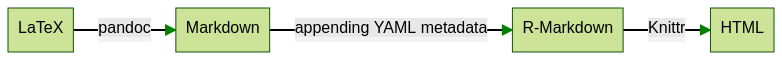
\includegraphics[width=1\textwidth]{figures/mermaid-diagram-20220417133810.png}
       \centering
      \textcolor{Orange}{\textbf{\caption{Process of Conversion}}}\label{fig:1}
    \end{figure}
The diagram here shows the flow of conversion of an article in LaTeX source file to HTML document.
The functions are supposed to invoke the pandoc conversion for the given file and export it in markdown.
Then take that markdown file convert it into R-Markdown by appending the YAML headers. Along with this the Function also needs to copy the supporting files such as bibliography, images etc. Lastly one can knit the R-Markdown into HTML file.

Although it is not perfect this process works out but there are potential issues such as file path handling, automation of reading the YAML header metadata information from the Tex File itself.\\
\\
{\large\bfseries Potential Challenges}
\begin{enumerate}[label = {  \color{MediumBlue} \textbf{\arabic*. }},align=left]
\item LateX conversion which includes pdf might not be rendered properly. I have to look into this and come up with a different strategy.
\item Automating the process of reading the tex file and adding the relevant YAML headers such as :
 title, author etc..
\end{enumerate}
 \subsubsection{8. TimeLine}
 {\textit{\textbf{Note:} This Timeline is a provisional timeline, the events and goals may change as per the circumstances.}}\\
{\large\bfseries {\color{orange}Today - April 19}  GSoC contributor application deadline}
\begin{enumerate}[label = {  \color{MediumBlue} \textbf{\arabic*. }},align=left]
\item Till April 19, I would complete the tests,contact mentors,finish the  proposal and take care of  formalities.
\end{enumerate}
{\large\bfseries {\color{orange}May 20 - June 12}  Community Bonding Period }
\begin{enumerate}[label = {  \color{MediumBlue} \textbf{\arabic*. }},align=left]
\item Increased communication with my mentor and co-mentor for more information and queries.
\item During this time frame I would like to interact and get to know more about the mentors, R community members and other GSoC contributors. 
\item One of my interests in discussion would be how is the R journal going to automate the process of conversion.
\item Going through rjtools package and getting up to speed with that
\item As I have described the coding plan above, I feel this time is the right time to discuss, do preliminary analysis and get more information on the articles, search for a diverse pool of articles to start my pilot run with. 
 \end{enumerate}
{\large\bfseries  {\color{orange}June 13 - June 30} Phase 1 - Pilot Testing}
\begin{enumerate}[label = {  \color{MediumBlue} \textbf{\arabic*. }},align=left]
\item Pilot test run of the existing code and analyzing the results.
\item Fixing bugs based on the initial tests.
\item Improvements in the R code with regards to implementation.
\item Inclusion of better vignette examples. 
\item Phase-1 Report Document by June 30.
\end{enumerate}
{\large\bfseries {\color{orange}June 30 - July 15} Phase 2 - Adding Test Suites}
\begin{enumerate}[label = {  \color{MediumBlue} \textbf{\arabic*. }},align=left]
\item Code Improvements, bug fixes.
\item Work on Test-Suites for Testing the code.
\item Completion of pending Phase-1 work (if any).
\item Phase-2 Report Document by July 16.
\end{enumerate}
{\large\bfseries {\color{orange}July 15 - July 30} Phase 3 - Documentation}
\begin{enumerate}[label = {  \color{MediumBlue} \textbf{\arabic*. }},align=left]
\item Adding Documentation, guided tutorials for the usage and conversion process.
\item Completion of pending work from previous phases (if any).
\item Conversion of articles by hand with special edits and inspection.
\item Draft Submission of GSoC Phase 1 Evaluation Report before July 25.
\item Phase-3 Report Document by July 31.
\end{enumerate}
{\large\bfseries {\color{orange}July 30 - August 15} Phase 4 - Work Period}
\begin{enumerate}[label = {  \color{MediumBlue} \textbf{\arabic*. }},align=left]
\item Considering this is the work period, I would take the project further with guidance from my mentors.
\item Proposed period where the final set of Functions along with documentation would be ready.
\item Completion of pending work from previous phases (if any).
\item Conversion of articles by hand with special edits and inspection.
\item Would like to get involved with the R journal team on how they plan to convert documents.
\item Phase-4 Report Document by August 16.
\end{enumerate}
{\large\bfseries {\color{orange}August 15 - August 30} Phase 5 - Automation}
\begin{enumerate}[label = {  \color{MediumBlue} \textbf{\arabic*. }},align=left]
\item Development of Automated Scripts for local conversion of a document from LaTeX to HTML.
\item Conversion of articles by hand with special edits and inspection.
\item Phase-5 Report Document by August 31.
\end{enumerate}
{\large\bfseries {\color{orange}August 30 - September 15} Phase 6 - Wrapping up}
\begin{enumerate}[label = {  \color{MediumBlue} \textbf{\arabic*. }},align=left]
\item drafting and submission of final work product and  final mentor evaluation.
\item Conversion of articles by hand with special edits and inspection.
\item Completing final checks and reviews.
\item Phase-6 Report Document by September 12
\end{enumerate}
{\large\bfseries {\color{orange}September 15 and beyond } Phase X - Contributor}
\begin{enumerate}[label = {  \color{MediumBlue} \textbf{\arabic*. }},align=left]
\item Contributing code and other relevant submissions to open source project of R.
\item Would be interested in maintaining the TexoR package if it is not integrated into the Rjtools.
\end{enumerate}
\subsubsection{9. Management of Coding Project}
{\large\bfseries How do you propose to ensure code is submitted / tested?}
\begin{enumerate}[label = {  \color{MediumBlue} \textbf{\arabic*. }},align=left]
 \item {\color{MediumBlue} Electricity}: I live in a region where there is 24/7 Electricity supply, hence there should not be any technical problems with that. 
 \item {\color{MediumBlue} Internet}: I have a Fibre optic internet service as well as Wireless mobile data(for backup), hence communication should not be an issue.
 \item {\color{MediumBlue} Device}: I have a desktop PC as well as a Laptop, hence software development and other tasks should not face any issue.
 \item {\color{MediumBlue} Other}: If any issue arises, I will contact the mentor,co-mentor or r-team member to resolve the problem at the earliest and ensure code is submitted.
\end{enumerate}
{\large\bfseries How often do you plan to commit?}
\begin{enumerate}[label = {  \color{MediumBlue} \textbf{\arabic*. }},align=left]
 \item {\color{MediumBlue} Major Code Commits}: 2-3 times a week (approx.., may vary as per workload)
 \item {\color{MediumBlue} Minor Code Commits}: Regular commits throughout the Internship
 \item {\color{MediumBlue} Bug Fixes}: As soon as the issue is resolved and verified. 
 \item {\color{MediumBlue} Testing}: Initially manual testing would be prevalent but with time automatic testing would be implemented.
 \item {\color{MediumBlue} Documentation}: Regular documentation and reports.
 \item{\color{MediumBlue} Communication}:  I would like to communicate with my mentors and other members several times a week through Email/slack/Video-Conferencing or other means.
\end{enumerate}
{\large\bfseries What changes in commit behavior would indicate a problem?}\\
\begin{enumerate}[label = {  \color{MediumBlue} \textbf{\arabic*. }},align=left]
 \item {\color{MediumBlue} No Commit in the past 2 weeks}: Unless there is prior request/explanation for this behaviour, It could indicate that I might be facing some problem (technical or otherwise).
 \item {\color{MediumBlue} No Communication for a week}: Lacking or no communication for more than a week would indicate a major issue, unless previously agreed.
\end{enumerate}
\subsubsection{10. Test Results}
I have completed all the tests to the best possible extent I could and have added the link to the bottom of the Github wiki page  \href{https://github.com/rstats-gsoc/gsoc2022/wiki/Converting-past-R-Journal-articles-to-HTML}{\color{orange}Converting past R Journal articles to HTML}.\\
\\
{\large\bfseries Explaination to the Tests :}\\
\begin{enumerate}[label = {  \color{MediumBlue} \textbf{\arabic*. }},align=left]
 \item {\color{MediumBlue} Test-1 EASY}:\\
 I have created the article using  rjtools::create\_article()  to generate a dummy article, then I have edited the content and updated YAML headers manually. Using the command rmarkdown::render() to generate HTML and LaTeX PDF files. 
 \item {\color{MediumBlue} Test-2 MEDIUM}:\\
 The next thing I have done is divided the whole process into 4 functions for better modular code and to allow manual intervention at every stage.
 
\begin{enumerate}[label = {  \color{MediumBlue} \textbf{\arabic*. }},align=left]
\item \textit{\color{DarkBlue}Convert\_To\_Markdown()} : This function converts the tex file as input into markdown by invoking pandoc.
   \begin{code}[enhanced,drop shadow]{R code}
Convert_To_Markdown<- function(input_file_path){
    path=dirname(input_file_path)
    old_working_directory=getwd()
    setwd(path)
    input_file=basename(input_file_path)
    md_file=paste(toString(tools::file_path_sans_ext(input_file)),".md",sep="")
    rmarkdown::pandoc_convert(input_file, to= "markdown",output = md_file)
    setwd(old_working_directory)
}
    \end{code}
\item \textit{\color{DarkBlue}Append\_Markdown\_Files()} : This function appends the YAML headers as per the parameters, also it can be used to append other headers, create a new directory output and create a new R-Markdown file as a combination of the generated Markdown file in previous process and the YAML headers appended on the top.
   \begin{code}[enhanced,drop shadow]{R code}
Append_Markdown_Files <- function(input_file_path,title,bib_file){
    input_file=basename(input_file_path)
    md_file = file(input_file_path,open="rt")
    md_file_content=readLines(md_file)
    yml_header="---"
    title_string="title:"
    sensitized_title=paste0('"', title, '"')
    newline_string="\n"
    bibliography_string="bibliography:"
    output_string="output:"
    output_spec="rjtools::rjournal_web_article"
    output_file_name=paste(dirname(input_file_path),"/output/",toString(tools::file_path_sans_ext(input_file)),".Rmd",sep="")
    dir.create(dirname(output_file_name),showWarnings = F)
    rmd_yml_additions= paste(yml_header,newline_string,title_string,sensitized_title,newline_string,bibliography_string,bib_file,newline_string,output_string,output_spec,newline_string, sep =" ")
    output_file = file(output_file_name, open="wt")
    writeLines(paste(rmd_yml_additions,""),con=output_file,useBytes = FALSE)
    writeLines(paste(yml_header,""),con=output_file,useBytes = FALSE)
    writeLines(paste(md_file_content,""),con=output_file,useBytes = FALSE)
    close.connection(md_file,type = "rt")
    close.connection(output_file,type = "wt")
}
    \end{code}
\item \textit{\color{DarkBlue}Copy\_Other\_Files()} : This function will copy dependent files and folders into the output directory, the folders are selected through a white-list of usual most commonly used extensions and figures. This white list can be edited as well down the line for more extensions.
  \begin{code}[enhanced,drop shadow]{R code}
Copy_Other_Files<-function(from_path){
    old_working_directory=getwd()
    setwd(from_path)
    dir_list=list.dirs(recursive = FALSE)
    possible_dirs=c("*_files" , "figures")
    target_dir=basename(dir_list[grep(paste(possible_dirs,collapse="|"),dir_list)])
    print(target_dir)
    dir.create(paste("output/",target_dir,sep=""),showWarnings = F)
    file.copy(list.files(target_dir, full.names = TRUE), paste("output/",target_dir,sep=""), recursive = TRUE)
    file_list=list.files(recursive = FALSE)
    extensions = c("*.png", "*.jpg", "*.bib")
    target_files = unique(grep(paste(extensions,collapse="|"), file_list, value=TRUE))
    print(target_files)
    file.copy(target_files,to = "output/", copy.mode = T, recursive=FALSE,)
    setwd(old_working_directory)
}
    \end{code}
\item \textit{\color{DarkBlue}Produce\_HTML()} : This last function does one task of rendering the R-markdown file into a HTML document. through rmarkdown:render() function.
 \begin{code}[enhanced,drop shadow]{R code}
Produce_HTML<-function(input_file_path){
    rmarkdown::render(input = input_file_path,output_format = "html_document")
}
    \end{code}
\item \textit{\color{DarkBlue}Calling the functions with appropriate parameters} :This will orchestrate the whole conversion process and can also be converted into a super function if required.
 \begin{code}[enhanced,drop shadow]{R code}
rjtools::create_article()
rmarkdown::render('rjarticle/quokka-bilby.Rmd',quiet = TRUE)
Convert_To_Markdown("rjarticle/RJwrapper.tex")# Appending YAML headers
Append_Markdown_Files("rjarticle/RJwrapper.md",title= "ToOoOlTiPs: An R Package for Customizable Tooltips in Interactive Graphics",bib_file = "RJreferences.bib")
Copy_Other_Files("rjarticle/")
Produce_HTML('rjarticle/output/RJwrapper.Rmd')
\end{code}
\end{enumerate}
Also I have tested these functions on the two examples which were also a criteria and I think the script has done a pretty good job of that.
 \item {\color{MediumBlue} Test-3 HARD}:
 In this Test I have done the following procedure: 
\begin{enumerate}[label = {  \color{MediumBlue} \textbf{\arabic*. }},align=left]
\item Create a R package in R studio
\item Initialize git repo
\item Create a github repo and link it with the local git repo
\item Added the functions in a file in R folder.
\item Generated roxygen2 skeleton for inline documentation and generated man pages through devtools
\item Updated the DESCRIPTION file and included dependencies.
\item Initialized vignettes through usethis::use\_vignette() and produced a small example vignette
\item Last built the package and ran R CMD check --as-cran check.
\end{enumerate}
This was about building the package.
\end{enumerate}
For the Verification of test and checking out the generated output I would strongly recommend the reader to look through the links and check out the generated files.\\
\\
{\large\bfseries Links To Test Results}
\begin{enumerate}[label = {  \color{MediumBlue} \textbf{\arabic*. }},align=left]
 \item {\color{MediumBlue} Test-1 EASY}: \href{https://github.com/Abhi-1U/GSoC_22_R_Converting-past-R-Journal-articles-to-HTML/tree/main/Test-1}{\color{orange}Source code}
 \item {\color{MediumBlue} Test-2 MEDIUM}: \href{https://github.com/Abhi-1U/GSoC_22_R_Converting-past-R-Journal-articles-to-HTML/tree/main/Test-2}{\color{orange}Source code}
 \item {\color{MediumBlue} Test-3 HARD}: \href{https://github.com/Abhi-1U/GSoC_22_R_Converting-past-R-Journal-articles-to-HTML/tree/main/Test-3}{\color{orange}Readme} \href{https://github.com/Abhi-1U/TexoR}{\color{orange}TexoR Package} 
\end{enumerate}
{\large\bfseries Related Work}\\
I have also build packages in other languages like python.
 \begin{enumerate}[label = {  \color{MediumBlue} \textbf{\arabic*. }},align=left]
 \item Pyrix: \href{https://github.com/Abhi-1U/pyrix}{\color{orange}Source code} 
 \item gitlas: \href{https://github.com/Abhi-1U/gitlas}{\color{orange}Source code} 
\end{enumerate}


% %-------------------------Content------------------------


\end{document}
